\section{Grammar}
\label{sec:grammar}

% DEBORA
Our LTAG/DUDES grammars consists of two parts: a domain-specific part obtained by extracting all relevant information from the ontology lexicon, and a domain-independent part created manually comprising closed-class expressions such as determiners, pronouns, copulative and auxiliary verbs.

\subsection{DOMAIN-SPECIFIC GRAMMAR}
Talking about the automatic generation of domain-specific grammar, we have created a couple of LTAG-DUDES for each lexicon entry and for all its different forms. The types of lexicon entry we encountered are: \textit{verbs, common nouns, proper nouns, prepositons and adjectives}.

\subsubsection{VERBS}\mbox{}\\
All the verbs of our ontology lexicon in \textit{lemon} format are transitive verbs with active voice and indicative mood. The tree and the semantic representation would thus look as follows:

\medskip
\begin{center}
	\captionof{figure}{Grammar entry for: "acquire"}
\begin{tabular}{ p{10em} p{10em} }
	\label{tbl:grammar.acquire}
	
	\begin{center}
		\begin{tikzpicture}
		\Tree [.S [.DP$_1\downarrow$ ] [.VP [.V acquire ] DP$_2\downarrow$ ] ]	
		\end{tikzpicture}
	\end{center}
	
	&

	\begin{center}
		\begin{tabular}{|c|l|}
			\hline
			\mbox{} & \mbox{}\\
			\hline
			\multicolumn{2}{|l|}{
				$isAcquiredBy(x,y)$
			} \\
			\hline
			\multicolumn{2}{|l|}{
				$(x,DP_{1}),(y,DP_{2})$
			} \\
			\hline
		\end{tabular}
	\end{center}	
	\\
\end{tabular}
\end{center}
\medskip

\subsubsection{NOUN ENTRIES}\mbox{}\\
In our ontology lexicon we can distinguish between common nouns, relational nouns and proper nouns. If the lexical entry of the ontology lexicon in \textit{lemon} has the tag \textit{possessiveAdjunct} we have a relational noun and the LTAG tree and DUDES would thus look as follows: 

\medskip
\begin{center}
	\captionof{figure}{Grammar entry for: "chairman of"}
\begin{tabular}{ p{10em} p{10em} }
	\label{tbl:grammar.chairmanOf}
	
	\begin{center}
		\begin{tikzpicture}
		\Tree [.NP [.N chairman ] [.PP [.P of ] DP$_1\downarrow$ ] ]
		\end{tikzpicture}
	\end{center}
		
	&
	
	\begin{center}
		\begin{tabular}{|c|l|}
			\hline
			y & \mbox{}\\ 
			\hline
			\multicolumn{2}{|l|}{
				$hasChairmanOf(x,y)$
			} \\
			\hline
			\multicolumn{2}{|l|}{
				$(x,DP_{1})$
			} \\
			\hline
		\end{tabular}
	\end{center}	
	\\
\end{tabular}
\end{center}
\medskip

Simple common nouns and proper nouns differ from relational nouns in their syntactic behaviour and sense. A common noun, as \textit{CEO, corporate officer}, and so on, has the following LTAG tree and DUDES:

\medskip
\begin{center}
	\captionof{figure}{Grammar entry for: "people"}
\begin{tabular}{ p{10em} p{10em} }
	\label{tbl:grammar.people}
	
	\begin{center}
		\begin{tikzpicture}
		\Tree [.NP people ]
		\end{tikzpicture}
	\end{center}
		
	&
	
	\begin{center}
		\begin{tabular}{|c|l|}
			\hline
			x & \mbox{}\\ 
			\hline
			\multicolumn{2}{|l|}{
				$Person(x)$
			} \\
			\hline
			\multicolumn{2}{|l|}{
				\mbox{}
			} \\
			\hline
		\end{tabular}
	\end{center}	
	\\
\end{tabular}
\end{center}
\medskip

A proper noun, as \textit{Microsoft, Google,} and so on, has instead the following LTAG tree and DUDES:
 
\medskip
\begin{center}
	\captionof{figure}{Grammar entry for: "Microsoft"}
\begin{tabular}{ p{10em} p{10em} }
	\label{tbl:grammar.microsoft}
	
	\begin{center}
		\begin{tikzpicture}
		\Tree [.DP Microsoft ]
		\end{tikzpicture}
	\end{center}
		
	&
	
	\begin{center}
		\begin{tabular}{|c|l|}
			\hline
			x & x\\ 
			\hline
			\multicolumn{2}{|l|}{
				$x=Microsoft$
			} \\
			\hline
			\multicolumn{2}{|l|}{
				\mbox{}
			} \\
			\hline
		\end{tabular}
	\end{center}	
	\\
\end{tabular}
\end{center}
\medskip

\subsubsection{ADJECTIVES}\mbox{}\\
We have different types of adjectives. Let's take some examples:
\begin{enumerate}
\item "\textit{an \textbf{italian} company}". In this case \textit{italian} is an \textbf{attributive} adjective and the associated grammar is the following:
 \medskip
\begin{center}
	\captionof{figure}{Grammar entry for: "italian" - attributive adjective}
\begin{tabular}{ p{10em} p{10em} }
	\label{tbl:grammar.attributiveAdjective}
	
	\begin{center}
		\begin{tikzpicture}
		\Tree [.NP [.ADJ italian ] [.NP$_1^\ast$ ] ]
		\end{tikzpicture}
	\end{center}
		
	&
	
	\begin{center}
		\begin{tabular}{|c|l|}
			\hline
			x & \mbox{}\\ 
			\hline
			\multicolumn{2}{|l|}{
				$hasNation(x,Italy)$
			} \\
			\hline
			\multicolumn{2}{|l|}{
				\mbox{}
			} \\
			\hline
		\end{tabular}
	\end{center}	
	\\
\end{tabular}
\end{center}
\medskip

\item "\textit{Is Satya Nadella \textbf{Italian}?}". In this example \textit{italian} is a  \textbf{predicative} adjective and the LTAG and DUDES are:
\medskip
\begin{center}
	\captionof{figure}{Grammar entry for: "italian" - predicative adjective}
\begin{tabular}{ p{10em} p{10em} }
	\label{tbl:grammar.predicativeAdjective}
	
	\begin{center}
		\begin{tikzpicture}
		\Tree [.DP  [.NP [.ADJ italian ] ] ]
		\end{tikzpicture}
	\end{center}
		
	&

	\begin{center}
		\begin{tabular}{|c|l|}
			\hline
			x & (x,y)\\ 
			\hline
			\multicolumn{2}{|l|}{
				$(y,Italy)=hasNation(x,y)$
			} \\
			\hline
			\multicolumn{2}{|l|}{
				\mbox{}
			} \\
			\hline
		\end{tabular}
	\end{center}	
	\\
\end{tabular}
\end{center}
\medskip
\item "\textit{heaquartered in Italy}". In this third case \textit{headquarterd} is a \textbf{prepositional} adjective. The grammar is the following:

\medskip
\begin{center}
	\captionof{figure}{Grammar entry for: "headquartered in"}
\begin{tabular}{ p{10em} p{10em} }
	\label{tbl:grammar.headquarteredIn}
	
	\begin{center}
		\begin{tikzpicture}
		\Tree [.NP [.NP$_1^\ast$ ] [.ADJPP [.ADJ headquartered ] [.PP [.P in ] DP$_1\downarrow$ ] ] ]	
		\end{tikzpicture}
	\end{center}
	
	&

	\begin{center}
		\begin{tabular}{|c|l|}
			\hline
			x & \mbox{}\\
			\hline
			\multicolumn{2}{|l|}{
				$hasHeadquarter(x,y)$
			} \\
			\hline
			\multicolumn{2}{|l|}{
				$(y,DP_{1})$
			} \\
			\hline
		\end{tabular}
	\end{center}	
	\\
\end{tabular}
\end{center}
\medskip
\end{enumerate}



\subsection{DOMAIN-INDEPENDENT GRAMMAR}
For the domain-independent expressions, we generate manually a fixed grammar entry for each word or expression we could encounter. For example we have generated a grammar for the expression \textit{how many}:
 \medskip
\begin{center}
	\captionof{figure}{Grammar entry for: "How many"}
\begin{tabular}{ p{10em} p{10em} }
	\label{tbl:grammar.howMany}
	
	\begin{center}
		\begin{tikzpicture}
		\Tree [.DP  [.PRNP [.ADV How ] [.PRN many ]] [.NP$_1\downarrow$ ]]
		\end{tikzpicture}
	\end{center}
		
	&
	%[.DP [.PRNP [ADV How] [PRN many] ] .NP$_1\downarrow$]
	\begin{center}
		\begin{tabular}{|c|l|}
			\hline
			x & x\\ 
			\hline
			\multicolumn{2}{|l|}{
				\mbox{}
			} \\
			\hline
			\multicolumn{2}{|l|}{
				$(x,NP_{1})$
			} \\
			\hline
		\end{tabular}
	\end{center}	
	\\
\end{tabular}
\end{center}
\medskip

????????? nel dudes bisogna inserire il "return: count(x)".??????????

The auxiliary verbs, as \textit{do, does, did, have, has, had}, don't have a semantic interpretation, so the DUDES is empty. The LTAG instead is in the form of adjunction tree:
\medskip
\begin{center}
	\captionof{figure}{Grammar entry for: "do"}
\begin{tabular}{ p{10em} p{10em} }
	\label{tbl:grammar.do}
	
	\begin{center}
		\begin{tikzpicture}
		\Tree [.S  [.V do ] [.S$_2^\ast$ ]]
		\end{tikzpicture}
	\end{center}
			
	\\
\end{tabular}
\end{center}
\medskip

We have generated grammar also for determiners, pronouns and copulative verbs. Determiners, i.e. \textit{the, a, an} has the following grammar:
\medskip
\begin{center}
	\captionof{figure}{Grammar entry for: "the"}
\begin{tabular}{ p{10em} p{10em} }
	\label{tbl:grammar.the}
	
	\begin{center}
		\begin{tikzpicture}
		\Tree [.DP  [.DET the ] [.NP$_1\downarrow$ ]]
		\end{tikzpicture}
	\end{center}
		
	&

	\begin{center}
		\begin{tabular}{|c|l|}
			\hline
			x & x\\ 
			\hline
			\multicolumn{2}{|l|}{
				\mbox{}
			} \\
			\hline
			\multicolumn{2}{|l|}{
				$(x,NP_{1})$
			} \\
			\hline
		\end{tabular}
	\end{center}	
	\\
\end{tabular}
\end{center}
\medskip

The grammar of wh-pronoun, as \textit{who, what, where}, is:
\medskip
\begin{center}
	\captionof{figure}{Grammar entry for: "who"}
\begin{tabular}{ p{10em} p{10em} }
	\label{tbl:grammar.who}
	
	\begin{center}
		\begin{tikzpicture}
		\Tree [.DP  [.PRN what ] ]
		\end{tikzpicture}
	\end{center}
		
	&

	\begin{center}
		\begin{tabular}{|c|l|}
			\hline
			x & x\\ 
			\hline
			\multicolumn{2}{|l|}{
				\mbox{}
			} \\
			\hline
			\multicolumn{2}{|l|}{
				\mbox{}
			} \\
			\hline
		\end{tabular}
	\end{center}	
	\\
\end{tabular}
\end{center}
\medskip

???????? nel duded da aggiungere il "return x"???????????

Finally, we have to considered the copulative verbs. They have two different syntactic representations, for example consider the following questions:
\begin{enumerate}
\item \textit{Where is Microsoft headquartered?}
\item \textit{Is Satya Nadella the CEO of Microsoft?}
\end{enumerate}
In the first case, the copulative verb \textit{is} has the grammar :
\medskip
\begin{center}
	\captionof{figure}{Grammar entry for: "is" (1)}
\begin{tabular}{ p{10em} p{10em} }
	\label{tbl:grammar.is}
	
	\begin{center}
		\begin{tikzpicture}
		\Tree [.S [.DP$_1\downarrow$ ] [.VP [.V is ] DP$_2\downarrow$ ] ]	
		\end{tikzpicture}
	\end{center}
	
	&

	\begin{center}
		\begin{tabular}{|c|l|}
			\hline
			\mbox{} & \mbox{}\\
			\hline
			\multicolumn{2}{|l|}{
				$replace(y,x)$
			} \\
			\hline
			\multicolumn{2}{|l|}{
				$(x,DP_{1}),(y,DP_{2})$
			} \\
			\hline
		\end{tabular}
	\end{center}	
	\\
\end{tabular}
\end{center}
\medskip

In the second case the grammar have to be the following:
\medskip
\begin{center}
	\captionof{figure}{Grammar entry for: "is" (2)}
\begin{tabular}{ p{10em} p{10em} }
	\label{tbl:grammar.is}
	
	\begin{center}
		\begin{tikzpicture}
		\Tree [.S [.VP [.V is ] DP$_1\downarrow$ ] [.DP$_2\downarrow$ ] ]	
		\end{tikzpicture}
	\end{center}
	
	&

	\begin{center}
		\begin{tabular}{|c|l|}
			\hline
			\mbox{} & \mbox{}\\
			\hline
			\multicolumn{2}{|l|}{
				$replace(y,x)$
			} \\
			\hline
			\multicolumn{2}{|l|}{
				$(x,DP_{1}),(y,DP_{2})$
			} \\
			\hline
		\end{tabular}
	\end{center}	
	\\
\end{tabular}
\end{center}
\medskip